\section{TRABALHOS RELACIONADOS}

%Trabalhos de mineração de textos (Lucas, Priscila, morais e ambrósio)
Explorar comentários de vídeos do Youtube é uma área de pesquisa recente e ainda em crescimento. Os trabalhos de \citeonline{ammari2011filteringYt} e \citeonline{schultes2013leave} são pesquisas relativamente recentes que possuem coleta, mineração e classificação desses comentários.

O trabalho de \citeonline{ammari2011filteringYt} faz parte de um grupo maior de pesquisas, que visam elaborar um modelo de usuário que possa ser utilizado em simuladores de aprendizagem. Seu foco é apresentar uma técnica de filtragem de comentários com baixo valor semântico para o domínio selecionado, coletados de mídias sociais. A técnica proposta combina aprendizagem de máquina, mineração de dados, e análise semântica, a fim de obter comentários que sejam relevantes para o domínio desejado. A construção do modelo foi feita utilizando os classificadores Naïve Bayes Multinomial e Árvore de Decisão C4.5.

\citeonline{ammari2011filteringYt} coletou 1159 comentários de 17 vídeos do Youtube, dos quais 5 vídeos tiveram 193 comentários selecionados para o grupo de controle do modelo. A técnica apresentada e utilizada por \citeonline{ammari2011filteringYt} é mostrada na Figura \ref{fig:ammari-metodologia}:

\begin{figure}[H] %use h para forçar que a figura fique abaixo do texto
	\caption{\label{fig:ammari-metodologia} Metodologia de filtragem para comentários de baixo valor semântico do Youtube.}
	\begin{center}
	    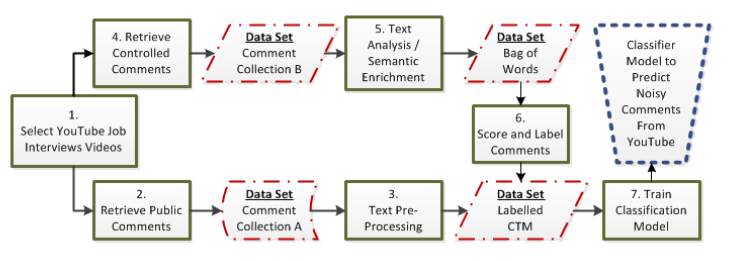
\includegraphics[scale=0.8]{figuras/figura_3.PNG} % altere o atributo scale para o tamanho da figura
	\end{center}
	\legend{Fonte: \citeonline{ammari2011filteringYt}}
\end{figure}

A metodologia da Figura \ref{fig:ammari-metodologia} consiste em:

\textbf{1.} Selecionar vídeos sobre entrevistas de emprego no Youtube.

\textbf{2.} Coletar os comentários públicos dos vídeos selecionados.

\textbf{3.} Pré-Processar os comentários obtidos.

\textbf{4.} Selecionar um grupo de comentários para grupo de controle, esses comentários são considerados relevantes para o domínio de entrevistas de emprego selecionado.

\textbf{5.} Analisar os comentários do grupo de controle, a fim de obter um Corpo de Palavras enriquecido semanticamente, relevante para o domínio.

\textcolor{red}{Parei aqui}

\textbf{6.} Pontuar os comentários para facilitar sua classificação, que no caso do trabalho de \citeonline{ammari2011filteringYt} é \textit{relevant} (relevante) ou \textit{noisy} (ruidoso - com baixo valor semântico).

\textbf{7.} Com os comentários devidamente pontuados, treinar um modelo de classificação supervisionado que irá indicar se um comentário é relevante ou não para o domínio proposto.

Os resultados apresentados por \citeonline{ammari2011filteringYt} indicam um alta taxa de acerto dos classificadores para os comentários obtidos e pré-processados com a metodologia proposta, sendo 86,7\% de corretude para o algoritmo C4.5 e 83,7\% para o Naïve Bayes Multinomial.

%Esse parágrafo vai pra tabela.
\begin{comment}
Sua principal diferença para este estudo é que apesar de focar inicialmente em vídeos infantis, este trabalho pretende ser capaz de aplicar o modelo em qualquer vídeo do Youtube, assim como em vídeos ao-vivo ou \textit{live-streaming}. Dessa forma, expandindo o domínio de aplicação. 
Este trabalho irá se utilizar de uma gama maior de comentários visto que o modelo de \citeonline{ammari2011filteringYt} foi testado apenas com 17 vídeos da plataforma e um total de 1159 comentários. Este trabalho pretende avaliar pelo menos 30 mil comentários de vídeos pertencentes a canais considerados de conteúdo infantil como \textbf{Telmo e Tula, desenhos animados} e \textbf{Galinha Pintadinha}, além de vídeos de programas infantis como \textbf{Peppa Pig} postados por usuários em canais diversos.
\end{comment}

\citeonline{schultes2013leave} afirmam em seu texto que comentários em vídeos do Youtube são, de forma geral, mal vistos pelo público: em uma pesquisa com 95 participantes, 64\% consideram comentários do Youtube "irrelevantes", 42\% consideram agressivos e 51\% os consideram "estúpidos", sendo que somente 6\% dos entrevistados consideram os comentários em vídeos do Youtube "De essencial importância". Por outro lado, \citeonline{schultes2013leave} também afirma que 34\% dos entrevistados leem os comentários dos vídeos e que 53\% lê os primeiros três comentários antes de começar a assistir o vídeo, além de estimar um total de 96 milhões de autores de comentários ativos na plataforma, chegando a conclusão de que a seção de comentários em vídeos do Youtube é uma funcionalidade essencial e uma das mais usadas em vídeos online. Levando esses fatores antagônicos em consideração, \citeonline{schultes2013leave} primeiramente procura verificar se comentários em vídeos do Youtube geram algum valor agregado e como medir esse valor, e acaba por provar que através dos comentários é também possível obter uma análise semântica do vídeo em questão. 

No período de 15/03/2012 à 21/03/2012, \citeonline{schultes2013leave} coletou um total de 136.854 comentário dentre 304 vídeos do Youtube de categorias variadas. Para tentar descobrir se os comentários agregam algum valor para o leitor, propôs agregá-los em três tipos de comentários:
\begin{itemize}
    \item \textbf{Discussão:} Comentários que geram debates dentre os usuários da plataforma;
    \item \textbf{Comentários inferiores:} Comentários com ofensas ou conteúdo irrelevante para o vídeo em questão; 
   \item \textbf{Comentários substanciais:} Comentários não ofensivos que contém informação relevante e estão relacionados com o tema do vídeo em questão.
\end{itemize}
Após definir os tipos de comentários, ainda foram definidos dez subtipos a fim de tornar a classificação mais concisa. % Esses 10 tipos foram omitidos a fim de manter a brevidade desse texto.
Durante a validação do seu \textit{Dataset}, \citeonline{schultes2013leave} concluiram que "não existe um tipo de comentário dominante em vídeos do Youtube" e também que "30\% dos comentários são do tipo \textbf{Comentários inferiores}, o que pode explicar a má impressão dos usuários em relação aos comentários em vídeos do Youtube.

%Mario falcao
Sobre proteção de crianças online, \citeonline{marioFalcao2016} aborda em sua pesquisa o problema da falta de acompanhamento por parte dos pais, quanto a utilização da internet por seus filhos. 

\citeonline{marioFalcao2016} propõe um sistema multiagente composto por agentes que coletaram e analisaram dados do Facebook. Os agentes trabalham juntos para trazer dados relevantes para o modelo de classificação, que auxilia em detectar casos de aliciamento infantil. O algoritmo utilizado para a classificação foi de árvore de decisão J48 \cite{quinlan1986induction}, implementado no WEKA, uma ferramenta de mineração de dados gratuita. O modelo foi validado com o perfil do Facebook de duas crianças, com o consentimento dos pais, e os resultados foram satisfatórios onde o modelo mostrou que uma das crianças apresentava-se em grupo de risco e estaria possivelmente sendo aliciada por adultos. 
Em comparação, o foco deste trabalho não é detectar possíveis aliciadores, mas sim determinar se a seção de comentários de um vídeo de Youtube é seguro para a criança que está assistindo o vídeo, sendo uma outra camada de proteção para as crianças. O trabalho de \citeonline{marioFalcao2016} também chegou a verificar a eficácia do seu modelo com outros algoritmos de classificação, entre eles o Naive Bayes que será utilizado neste trabalho.

%EnyoGonçalves
\citeonline{EnyoGoncalves2017} extende o trabalho de \citeonline{marioFalcao2016} buscando detectar automaticamente quando uma mensagem suspeita é trocada entre uma criança e um adulto. O algoritmo de classificação utilizado é Naive Bayes Multinomial \cite{metsis2006spamBayes}.

Os dados utilizados para treinar o modelo com mensagens "perigosas" foram coletados do site: \footnote{http://www.perverted-justice.com}. Os dados com mensagens consideradas "normais" foram retirados do site: \footnote{http://vircio.net}. Foram utilizadas 1610 mensagens ao todo, com um total de 9450 palavras, para as quais o Naive Bayes Multinomial obteve uma taxa de acerto de 86,33\%. Após aplicar o modelo em conversa real entre uma criança e um suspeito de aliciamento, \citeonline{EnyoGoncalves2017} mostrou que seu modelo é mais robusto que o de \citeonline{marioFalcao2016}, pois pode detectar frases de aliciadores fora de contexto e além disso, detecta frases como um todo e não somente palavras-chave.

A tabela a seguir, apresenta uma comparação entres os trabalhos citados anteriormente e este trabalho em questão:
% eu poderia fazer duas tabelas (uma pra os dois de mineração e uma para os do marcos antonio) maybe
\begin{table}[H]
	\Caption{\label{tabela-trabalhos} Dados de coletas de comentários realizadas}%
	{%
		\begin{tabular}{p{3cm}ccp{4.5cm}} %{p{3cm}ccp{4.5cm}} não fica maior que o texto, horizontalmente
			\toprule
			Trabalho & Mineração de Texto & Proteção de crianças &  Objetivo\\
			\midrule \midrule
    		\cite{ammari2011filteringYt} & Sim & Não & Filtrar comentários do Youtube com pouco valor semântico.\\
    		\hline	
			\cite{schultes2013leave} & Sim & Não & Verificar a relevância de comentários do Youtube.\\
			\hline
			\cite{marioFalcao2016} & Sim & Sim & Medir nível de exposição de crianças no Facebook.\\
			\hline
			\cite{EnyoGoncalves2017} & Não & Sim & Detectar facilmente aliciadores de crianças na internet.\\
			\hline
			Este trabalho & Sim & Sim & Verificar se um comentário de vídeo do Youtube é adequado ou não para crianças.\\
			\bottomrule
		\end{tabular}%
	}{%
	\Fonte{Elaborado pelo autor}
}
\end{table}